\chapter{Introduction} 

\section{Background}

\subsection{Mobile Ad Hoc Networks}
A mobile ad hoc network (MANET),  is a self-configuring mesh network of mobile devices connected by wireless links.  
These mobile devices are free to move independently in any direction and it acts as a router, where it must forward traffic unrelated to its own use.

\subsection{Partitioned Networks}
Partitioned networks are networks with no single hop or multiple hop route between some or even all node pairs. %TODO: Cite?
In a partitioned network, nodes may remain fully disconnected or they may \emph{cluster}, forming subnetworks in which all nodes are connected.
All current used routing algorithms used in MANETs %TODO: list algorithms?
fail in the presence of partitioning ~\cite{Routing}.

\subsection{Delay and Loss Tolerant Networks}
\label{sec:delay_loss_tolerant}
%This section is pretty lame
A delay tolerant network is one in which there may be significant delay delivering packets.
This delay may range from a few minutes up to hours or even days. %cite
%TODO: reason - intermittently connected
Loss tolerant networks are networks in which a significant number of packets may be lost.

\subsection{Message Ferrying \& Store-Carry-Forward Routing}
\label{sec:ferrying_overview}
Message ferrying is the concept of making use of mobile nodes in a MANET networks to deliver data ~\cite{adhocmsgferry}.
Store-carry-forward routing is a strategy which makes use of known or assigned trajectories of these mobile nodes, known as message ferries, collect and deliver data.
Some messages are dropped if no route to the destination can be found.  
Message ferrying allows the message to buffer and carry messages until the connection is available to forward.

%TODO: include
%	- task vs message oriented ferries

%TODO HIPRI: ways message ferrying is used

\section{Motivations and Potential Applications}

%TODO: redo
%Main idea
%	- Many mobile devices - potentially many ferries
%	- Non-essential monitoring applications are delay and loss tolerant

With the continuous growth of today's mobile devices, such as smartphones, laptops, tablets, netbooks, and more, demands for different services are prominent. 
%The idea is to implement integrated intelligence for networked machine monitoring and controlling.
Some of these applications are integrated intelligence for networked monitoring and controllability between machines, track road traffic conditions, in-house utility management, automation for home devices, industrial monitoring applications, robot to robot communication and more.  
The use of these mesh networks must have low-cost, very low power consumption,low data rate, cheap installation, flexibility, and increase connectivity to make it worthwhile in most cases.

\section{Project Goals}

Message ferrying has typically been examined within the context of improving throughput, reducing delay and increasing reliability within a ad hoc network.
Due to the complexity of incorporating message ferrying into existing ad hoc routing algorithms, this project will focus on a network in which data is transported strictly using ferries.
No clustering of network nodes and routing within subnetworks will be considered.
Surprisingly, very little research has been found for a network with these characteristics.
The goals of this project may be listed as follows.

\begin{itemize}
\item Design and implement a message ferrying algorithm.
\item Simulate this algorithm in a highly partitioned network.
\item Evaluate the network based on delay and loss.
\item Examine the impact of node density and ferry count on the network.
\end{itemize}

%Research and implement a mesh network design with varying distances using ZigBee protocol and examine the feasibility for different applications.


%testingstuff
%\section{Section 1}
%\label{sec:sec-1}
%
%Citation ~\cite{book1}.
%Reference to section 1: \ref{sec:sec-1}
%
%
%
%
%An overview look of our architecture:
%
%\begin{figure}[h]
%    \centering
%    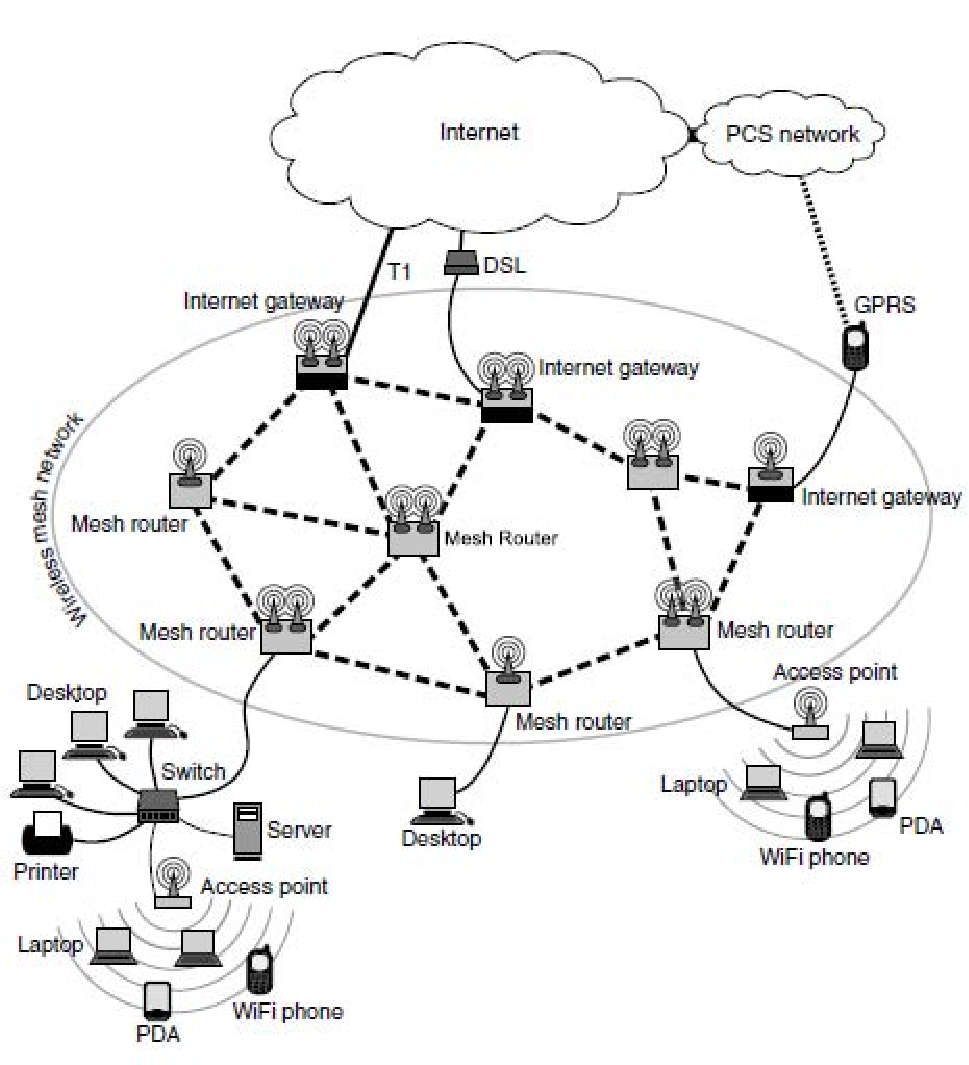
\includegraphics[width=.5\textwidth]{images/wmn_general}
%    \caption{Wireless Mesh Network General Architecture Overview~\cite{book1}}
%    \label{fig:wmn_general}
%\end{figure}
%
%if something referring to this figure, use this \ref{fig:wmn_general}
%
%Testing; just making references show
%asdf ~\cite{wearable}.
%asdf ~\cite{adhocmsgferry}.
%asdf ~\cite{hybrid}.
%asdf ~\cite{QoSrouting}.
%asdf ~\cite{efficientrouting}.
%asdf ~\cite{implement}.
%asdf ~\cite{book1}.